\section{Solution}

ResCred (See \autoref{fig:ResCred_description}) is a decentralized web application that utilizes ResilientDB to create a public blockchain to store, verify, and manage credentials, offering:
\begin{enumerate}
    \item Secure Verification \\
        We aim to be able to verify any transaction record in the database via any replica, using asymmetric cryptography to confirm the authenticity of the issuing body.
    \item Efficiency \\
        Automated verification process removes intermediaries from the issuing and verification process, improving reliability and the timeliness of verifying credentials.
    \item Transparency \\
        All transactions on ResCred are logged immutably which prevents tampering of records ensuring trust and accountability.
\end{enumerate}
Each certification will be recorded on ResilientDB as a transaction between an issuing body and a credential holder, allowing anyone to see the issuing and modification history of that record. Only authorized institutions will have the ability to issue, expire, or revoke credentials while remaining publicly accessible and verifiable.

\begin{figure}
    \begin{center}
        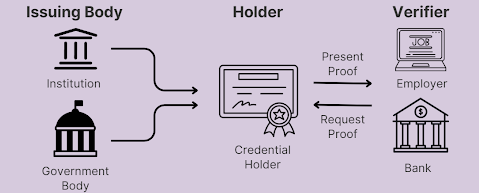
\includegraphics[width=0.95\textwidth]{img/rescred_description.png}
    \end{center}
    \caption{Picture describing ResCred}\label{fig:ResCred_description}
\end{figure}

